\documentclass[a4paper,10pt]{article}

\usepackage[utf8]{inputenc}
%\usepackage[T1]{fontenc}

\usepackage{textcomp}           % Extra Symbole (Grad Celsius etc.)
\usepackage{amssymb,amsmath}    % Schöne Formeln (AMS = American Mathematical Society)
\usepackage{graphicx}           % Bilder und Seitenränder
\usepackage{subcaption}			% captions for subfigures
\usepackage{booktabs}           % Schönere Tabellen
\usepackage{colortbl}           % Farbige Tabellen

%\usepackage{tcolorbox}			% schöne bunte Boxen
\usepackage{mathtools}			% \mathclap für ordentliche \underbrace-			environments
\usepackage[left=2cm,right=2cm,top=2cm,bottom=2cm]{geometry}			% Pagelayout mit \newgeometry, \restoregeometry
\usepackage{float}
\usepackage{wrapfig}
\usepackage{enumitem}
\usepackage{float}
\usepackage{braket}
\usepackage{caption}
\usepackage[per-mode=reciprocal,output-decimal-marker={.},binary-units=true,separate-uncertainty=true]{siunitx}
\usepackage[breaklinks=true,colorlinks=true,linkcolor=blue,urlcolor=blue,citecolor=blue]{hyperref}
\usepackage{physics}
\usepackage{url}
\usepackage{subcaption}
\usepackage{calrsfs}
\DeclareMathAlphabet{\pazocal}{OMS}{zplm}{m}{n}
\usepackage{tikz}
\usetikzlibrary{decorations, positioning, intersections, calc, shapes,arrows, scopes}
\usepackage{pgfplots}
\usepackage{bodegraph}
\usepackage{circuitikz}
\graphicspath{{./img/}}

\newcommand{\dif}{\mathrm{d}}

\bibliographystyle{unsrtnat}

\renewcommand{\k}{\mathbf{k}}
\begin{document}
\begin{titlepage}
 \begin{center}
	\Large{Advanced laboratory course 3}
	\end{center}
	\begin{center}
	 \LARGE{\textbf{FP3 - Electronic Controller}}
	\end{center}

	\begin{center}

	\large Marco \textsc{Canteri} \\
	marco.canteri@student.uibk.ac.at\\
	\large Maximilian \textsc{Münst} \\
	maximilian.muenst@student.uibk.ac.at
	\end{center}

	\begin{center}
	\vspace{1cm}
	Innsbruck, \today
	\vspace{1cm}
	\end{center}

	\begin{abstract}
    The main task of this experiment was to solder a PID-controller to regulate the temperature of a laser cavity in order to improve the stabilization of the laser.
  \end{abstract}
    \vspace{1cm}

	\begin{center}
	
\includegraphics[scale=0.4]{img/uibk}
	\end{center}

\end{titlepage}


\section{Introduction}
The ability to control and modulate the output of a system or process in a precise way is of fundamental importance not only in modern day science, but also in engineering and high-tech industry. The PID-controller, which was explored in this experiment, is a comparably simple, yet reliable and useful example for a controller. In this case it was used to stabilize the frequency of a He-Ne laser.

\section{Theoretical Background}
\label{theory}
\subsection{The Control Loop}
In this experiment we used a feedback loop, which is sketched in Fig. \ref{fig_control_loop}. The output of the system $X$ is the difference in intensity of two laser modes. It is compared to the desired value $W$. Their difference $W-X$, called error signal is fed into the controller, which is composed by three parts: a Proportional controller, a Integral controller, and Differential controller. The output of the controller $Y$ drives an heating coil which heat the He-Ne laser's cavity. The temperature is further influenced by outside influence, which is accounted by the error signal $Z$. The combined change in temperature causes the optical length of the cavity to change, thus changing the ratio in the intensities of the modes. This then leads back to a different output of the system, which closes the loop.
\begin{figure}[htp!]
    \centering
    \tikzstyle{block} = [draw, fill=blue!20, rectangle,
    minimum height=3em, minimum width=6em]
    \tikzstyle{sum} = [draw, fill=blue!20, circle, node distance=1cm]
    \tikzstyle{input} = [coordinate]
    \tikzstyle{output} = [coordinate]
    \tikzstyle{pinstyle} = [pin edge={to-,thin,black}]

\begin{tikzpicture}[auto, node distance=2cm,>=latex']
    \node [input, name=input] {};
    \node [sum, right of=input] (sum) {};
    \node [block, right of=sum,
            node distance=3cm] (system) {System ($A_S$)};
    \node [sum, right of=system, node distance=3cm, pin={[pinstyle]above:$W$}] (output) {};
    \node [block, below of=system] (controller) {Controller ($A_R$)};

    \draw [draw,->] (input) -- node {$Z$} (sum);
    \draw [->] (sum) -- node {$Y + Z$} (system);
    \draw [->] (system) --  node {$X$}(output);
    \draw [->] (output) |- node[pos=0.01] {$-$} node {$W - X$} (controller);
    \draw [->] (controller) -| node[pos=0.99] {$+$}
        node [near end] {$Y$} (sum);
\end{tikzpicture}
\caption{Sketch of a control loop. The output of the system $X$ is compared to the reference $W$. The difference in the signal is fed back into the controller. The output of the controller is the signal $Y$, which is added to the error value $Z$ and fed back into the system. }
\label{fig_control_loop}
\end{figure}

\subsection{Stabilizing the Laser}
The length of the cavity of the He-Ne laser only allows for two modes to reach a notable amount of amplification in the amplification profile. Fig. \ref{fig_profile} shows the profile and the two modes in the desired intensity ratio. These two modes are orthogonally polarized,due to non-linear mode competition in the cavity.\cite{laserfaq} Using a polarizing beam splitter, these modes are split up and are detected on individual photodiodes.

\begin{figure}[htp!]
  \centering
  \pgfmathdeclarefunction{gauss}{2}{%
  \pgfmathparse{1/(#2*sqrt(2*pi))*exp(-((x-#1)^2)/(2*#2^2))}%
  }
  \begin{tikzpicture}
    \begin{axis}[
      no markers, domain=0:10, samples=100, axis lines*=left, xlabel=Frequency at $\approx$\SI{633}{\nano \meter}, ylabel=Amplification,
      every axis y label/.style={at=(current axis.above origin),anchor=south},
      every axis x label/.style={at=(current axis.right of origin),anchor=west},
      height=5cm, width=12cm, xtickmax= 3,
      xtick=\empty, ytick=\empty, enlargelimits=false, clip=false, axis on top, grid = major
      ]
      \addplot [very thick,cyan!50!black] {gauss(5,1)};
      \draw [yshift=-0.6cm, latex-latex](axis cs:4,0) -- node [fill=white] {FSR} (axis cs:6,0);
      \draw (axis cs:4,0) -- (axis cs:4,0.24);
      \draw (axis cs:6,0) -- (axis cs:6,0.24);
    \end{axis}
  \end{tikzpicture}
  \caption{Sketch of the amplification profile including two laser modes. According to \cite{script} the FWHM of the amplifictaion profile is \SI{1.4}{\giga \hertz}, while the Free Spectral Range of the longitudinal modes is \SI{1.1}{\giga \hertz}. The modes are here shown with equal amplification, which is the situation that is to be reached with the controller.}
  \label{fig_profile}
\end{figure}
The aim is to have equal measured intensities on both photo diodes. This is accomplished by stabilizing the temperature of the laser's cavity at a point where the modes have equal intensities.

\subsection{P-Controller}
As is stated in \cite{script}, there are 3 types of controllers that are important to this experiment. The \textbf{P-Controller} (proportional), the \textbf{PI-Controller} (proportional-integral), and the \textbf{PID-Controller} (proportional-integral-differential). In this section a quick look is taken at the P-controller, the others are examined in the following sections.
\newline
To put it simply, the P-controller is a inverting linear amplifier. There is no notable phase change in the system caused by the P-controller. Fig. \ref{fig_bode_p} showcases the bode plot of a system consisting of three low-pass filters with breaking point frequencies at $f_1 = \SI{100}{\hertz}$, $f_2 = \SI{1}{\kilo \hertz}$, and $f_3 = \SI{10}{\kilo\hertz}$, that is connected to a P-controller. Our system is a low-pass since we are controlling the temperature, i.e. the system has to thermalize, which takes time.
\newline
The phase is untouched by the proportional controller and the amplitude of the system is increased all over the system by a constant factor. At the  critical frequency $f_k$, where the amplitude passes through \SI{0}{\decibel}, the difference between the phase and \SI{180}{\degree} should be around $\alpha = \SI{60}{\degree}$, because at this frequency the overshooting of the function should be only $4\%$ of the original amplitude at minimal equilibration time.\cite{halbleiter} If the phase is bigger than \SI{180}{\degree} at \SI{0}{\decibel}, then the system starts to oscillate. As the P-controller leaves a small deviation from the desired value, we have to add an integrator.

\begin{figure}[htp!]
  \centering
  \pgfdeclarelayer{background}
  \pgfdeclarelayer{foreground}
  \pgfsetlayers{background,main,foreground}
  \begin{tikzpicture}[>=latex',
    ref lines/.style={thin, black!60},
    ref points/.style={circle, black, opacity=0.7, fill, minimum size= 3pt, inner sep=0},
    every node/.style={font=\small},
    bode lines/.style={very thick, blue},
    Gclabel/.style={text=blue},
    xscale=12/12,
    gnuplot def/.style={samples=100,id=\arabic{idGnuplot},prefix=gnuplot/\jobname },
    semilog lines/.style={thin, black!60},
    semilog lines 2/.style={thin, black!20, dashed},
    semilog half lines/.style={semilog lines 2, dashed },
    Black lines/.style={very thick, blue},
    Black grid/.style={ultra thin,brown},
    Black abaque mag/.style={gray,ultra thin,dashed,smooth},
    Black abaque phase/.style={gray,ultra thin,smooth},
    Black label points/.style={font=\tiny},
    Black label axes/.style={Black grid, font=\tiny},
    Nyquist lines/.style={very thick, blue},
    Nyquist grid/.style={ultra thin,brown},
    Nyquist label axes/.style={Nyquist grid,font=\tiny},
    Nyquist label points/.style={font=\tiny},
    Temp lines/.style={very thick, blue},
    Temp grid/.style={ultra thin,brown},
    Temp label axes/.style={Temp grid, font=\tiny},
    Temp label points/.style={font=\tiny},
    Abaque grid/.style={ultra thin,brown!80},
    Abaque lines/.style={thick, blue,smooth},
    gnuplot def/.append style={prefix={}},
    ]
  \begin{scope}[xscale = 1.7, yscale=2.5/110]
    \UnitedB
    \semilog{0}{6}{-70}{80}
    \BodeAmp[bode lines, red, name path=Gomagnitude]{0:4.1}{
    + \KAmp{10}
    + \POAmp{1}{0.01}
    + \POAmp{1}{0.001}
    + \POAmp{1}{0.0001}
    }
    \node [rotate=90] at (-0.6, 5) {$A$ / \si{\decibel}};
  \end{scope}

  \begin{scope}[xshift=0cm,yshift=-2cm, xscale= 1.7, yscale=1.39/110]
\semilog{0}{6}{-270}{0}
\BodeArg[bode lines, red, name path=Gomagnitude]{0:6}{
+ \KArg{10}
+ \POArg{1}{0.01}
+ \POArg{1}{0.001}
+ \POArg{1}{0.0001}
}

\draw[<->] (2.85,-180) -- node {$\alpha = \SI{60}{\degree}$}(2.85,-120);
\node at (3,-330) {$f$ / \si{\hertz}};
\node [rotate=90] at (-0.6,-150) {$\varphi$ in \si{\degree}};
\end{scope}
\end{tikzpicture}
\caption{Bode plot of a P-controller and a serially attached system consisting of three low-pass filters with cut-off frequencies at $f_1 = \SI{100}{\hertz}$, $f_2 = \SI{1}{\kilo \hertz}$, and $f_3 = \SI{10}{\kilo\hertz}$. The arrow in the phase plot shows the phase reserve $\alpha$. }
\label{fig_bode_p}
\end{figure}

\begin{figure}
  \centering
  \begin{circuitikz}
    \draw
    (0, 0) node[op amp] (opamp) {}
    (opamp.-) to[generic=$R_{P1}$] (-3, 0.5) to[short, -o] (-3, 0.5) node[anchor=east] {$U_{in}$}
    (opamp.-) to[short,*-] ++(0,1.5) coordinate (leftC)
    to[generic=$R_{P2}$] (leftC -| opamp.out)
    to[short,-*] (opamp.out)
    (opamp.out) to[short, -o] (2, 0) node[anchor=west] {$U_{out}$}
    (opamp.+) |- (-1.5,-0.5) node[ground]{}
  ;\end{circuitikz}

  \begin{circuitikz}
    \draw
    (0, 0) node[op amp] (opamp) {}
    (opamp.-) to[generic=$R_{I}$] (-3, 0.5) to[short, -o] (-3, 0.5) node[anchor=east] {$U_{in}$}
    (opamp.-) to[short,*-] ++(0,1.5) coordinate (leftC)
    to[capacitor=$C_{I}$] (leftC -| opamp.out)
    to[short,-*] (opamp.out)
    (opamp.out) to[short, -o] (2, 0) node[anchor=west] {$U_{out}$}
    (opamp.+) |- (-1.5,-0.5) node[ground]{}
  ;\end{circuitikz}

  \begin{circuitikz}
    \draw
    (0, 0) node[op amp] (opamp) {}
    (opamp.-) to[capacitor=$C_{D}$] (-3, 0.5) to[short, -o] (-3, 0.5) node[anchor=east] {$U_{in}$}
    (opamp.-) to[short,*-] ++(0,1.5) coordinate (leftC)
    to[generic=$R_{D}$] (leftC -| opamp.out)
    to[short,-*] (opamp.out)
    (opamp.out) to[short, -o] (2, 0) node[anchor=west] {$U_{out}$}
    (opamp.+) |- (-1.5,-0.5) node[ground]{}
  ;\end{circuitikz}

  \caption{Circuit diagrams of a P-controller (first), a I-part (middle), and a D-part (bottom). To get a PID-controller, one has to arrange them in a parallel way. }
  \label{fig_circuit_p}
\end{figure}

\subsection{PI-Controller}
The bode plot of the PI-controller is shown in Fig. \ref{fig_bode_pi}. As one can see the amplitude rises at low frequencies, thus decreases the deviation from the desired value. The cutoff frequency of the controller should be chosen to be
\begin{equation}
  f_I = \frac{1}{2 \pi C_{\mathrm{PI}} R_{\mathrm{PI}}}\approx \frac{1}{10} f_k,
\end{equation}
where $f_k$ is the critical frequency of the proportional controller. Also, the phase is hardly changed at the critical temperature, which means that $\alpha$ should remain unchanged. To flatten out the phase at the critical frequency one can add a differential controller.
\begin{figure}[htp!]
  \centering
  \pgfdeclarelayer{background}
  \pgfdeclarelayer{foreground}
  \pgfsetlayers{background,main,foreground}
  \begin{tikzpicture}[>=latex',
    ref lines/.style={thin, black!60},
    ref points/.style={circle, black, opacity=0.7, fill, minimum size= 3pt, inner sep=0},
    every node/.style={font=\small},
    bode lines/.style={very thick, blue},
    Gclabel/.style={text=blue},
    xscale=12/12,
    gnuplot def/.style={samples=100,id=\arabic{idGnuplot},prefix=gnuplot/\jobname },
    semilog lines/.style={thin, black!60},
    semilog lines 2/.style={thin, black!20, dashed},
    semilog half lines/.style={semilog lines 2, dashed },
    Black lines/.style={very thick, blue},
    Black grid/.style={ultra thin,brown},
    Black abaque mag/.style={gray,ultra thin,dashed,smooth},
    Black abaque phase/.style={gray,ultra thin,smooth},
    Black label points/.style={font=\tiny},
    Black label axes/.style={Black grid, font=\tiny},
    Nyquist lines/.style={very thick, blue},
    Nyquist grid/.style={ultra thin,brown},
    Nyquist label axes/.style={Nyquist grid,font=\tiny},
    Nyquist label points/.style={font=\tiny},
    Temp lines/.style={very thick, blue},
    Temp grid/.style={ultra thin,brown},
    Temp label axes/.style={Temp grid, font=\tiny},
    Temp label points/.style={font=\tiny},
    Abaque grid/.style={ultra thin,brown!80},
    Abaque lines/.style={thick, blue,smooth},
    gnuplot def/.append style={prefix={}},
    ]
    \begin{scope}[xscale = 1.7, yscale=2.5/110]
      \UnitedB
      \semilog{0}{6}{-70}{80}
    \BodeAmp[bode lines, red, name path=Gomagnitude]{0:4.1}{
    + \POAmp{1}{0.01}
    + \POAmp{1}{0.001}
    + \POAmp{1}{0.0001}
    + \PIAmp{10}{0.01}
    }
    \node [rotate=90] at (-0.6, 5) {$A$ / \si{\decibel}};
  \end{scope}

  \begin{scope}[xshift=0cm,yshift=-2cm, xscale= 1.7, yscale=1.39/110]
\semilog{0}{6}{-270}{0}
\BodeArg[bode lines, red, name path=Gomagnitude]{0:6}{
+ \POArg{1}{0.01}
+ \POArg{1}{0.001}
+ \POArg{1}{0.0001}
+ \PIArg{10}{0.01}
}

\draw[<->] (2.75,-180) -- node {$\alpha = \SI{60}{\degree}$}(2.75,-120);
\node at (3,-330) {$f$ / \si{\hertz}};
\node [rotate=90] at (-0.6,-150) {$\varphi$ in \si{\degree}};
\end{scope}
\end{tikzpicture}
\caption{Bode plots of a PI-controller to which the system is serially connected. Again the parameters were chosen so that the phase reserve is about \SI{60}{\degree}.}
\label{fig_bode_pi}
\end{figure}

\subsection{PID-Controller}
For the final part a differential controller is added. The result can be seen in Fig. \ref{fig_bode_pid}. The rising edge frequency of the differential controller should be set to
\begin{equation}
  f_I = \frac{1}{2 \pi C_\mathrm{D} R_\mathrm{D}} \approx f_k,
\end{equation}
while the frequency of the integrator stays at a tenth of the critical frequency $f_k$.
\begin{figure}[htp!]
  \centering
  \pgfdeclarelayer{background}
  \pgfdeclarelayer{foreground}
  \pgfsetlayers{background,main,foreground}
  \begin{tikzpicture}[>=latex',
    ref lines/.style={thin, black!60},
    ref points/.style={circle, black, opacity=0.7, fill, minimum size= 3pt, inner sep=0},
    every node/.style={font=\small},
    bode lines/.style={very thick, blue},
    Gclabel/.style={text=blue},
    xscale=12/12,
    gnuplot def/.style={samples=100,id=\arabic{idGnuplot},prefix=gnuplot/\jobname },
    semilog lines/.style={thin, black!60},
    semilog lines 2/.style={thin, black!20, dashed},
    semilog half lines/.style={semilog lines 2, dashed },
    Black lines/.style={very thick, blue},
    Black grid/.style={ultra thin,brown},
    Black abaque mag/.style={gray,ultra thin,dashed,smooth},
    Black abaque phase/.style={gray,ultra thin,smooth},
    Black label points/.style={font=\tiny},
    Black label axes/.style={Black grid, font=\tiny},
    Nyquist lines/.style={very thick, blue},
    Nyquist grid/.style={ultra thin,brown},
    Nyquist label axes/.style={Nyquist grid,font=\tiny},
    Nyquist label points/.style={font=\tiny},
    Temp lines/.style={very thick, blue},
    Temp grid/.style={ultra thin,brown},
    Temp label axes/.style={Temp grid, font=\tiny},
    Temp label points/.style={font=\tiny},
    Abaque grid/.style={ultra thin,brown!80},
    Abaque lines/.style={thick, blue,smooth},
    gnuplot def/.append style={prefix={}},
    ]
    \begin{scope}[xscale = 1.7, yscale=2.5/110]
      \UnitedB
      \semilog{0}{6}{-70}{80}
    \BodeAmp[bode lines, red, name path=Gomagnitude]{0:5}{
    + \POAmp{1}{0.01}
    + \POAmp{1}{0.001}
    + \POAmp{1}{0.0001}
    + \PIDAmp{100}{0.01}{0.0007}
    }
    \node [rotate=90] at (-0.6, 5) {$A$ / \si{\decibel}};
  \end{scope}

  \begin{scope}[xshift=0cm,yshift=-2cm, xscale= 1.7, yscale=1.39/110]
\semilog{0}{6}{-270}{0}
\BodeArg[bode lines, red, name path=Gomagnitude]{0:6}{
+ \POArg{1}{0.01}
+ \POArg{1}{0.001}
+ \POArg{1}{0.0001}
+ \PIDArg{10}{0.01}{0.0007}
}

\draw[<->] (3.7,-180) -- node {$\alpha = \SI{60}{\degree}$}(3.7,-120);
\node at (3,-330) {$f$ / \si{\hertz}};
\node [rotate=90] at (-0.6,-150) {$\varphi$ in \si{\degree}};
\end{scope}
\end{tikzpicture}
\caption{Bode plots of the series of a PID-controller and the system. As one can see, the phase curve is flatter than in the previous examples. }
\label{fig_bode_pid}
\end{figure}

\section{Experimental Setup}
\subsection{The Optical Setup}
The central part of the setup is the He-Ne laser. Beams can exit its cavity on both ends, which means there are two beams to be observed. One is lead into a Fabry-Perot etalon in order to examine the frequency difference of the two generated modes, which gives us a gauge for the frequency axis. Also from the movement of the peaks in the peaks in the output of the Fabry-Perot interferometer, we can determine the stability of the used controller.
\newline
The second beam of the He-Ne laser is split on a polarizing beam splitter. Since the two modes of the laser are orthogonal, it is possible to separate the modes. The intensities of both modes are then analyzed by making use of two individual photodiodes. Their signal is then fed into the controller to determine the appropriate amount of heating necessary to stabilize the two laser modes and thus stabilize the laser.
% we need a sketch of the setup here, should we copy and photoshop the one from the script or make a new one?
\begin{figure}[htp!]
    \centering
    \tikzstyle{laser} = [draw, fill=red!20, rectangle,
    minimum height=3em, minimum width=6em]
    \tikzstyle{pbs} = [draw, fill=blue!20, rectangle, minimum height=3em, minimum width=3em]
    \tikzstyle{pd} = [draw, fill = gray!20, rectangle, minimum height=0.5em, minimum width=1em]
    \tikzstyle{output} = [coordinate]
    \tikzstyle{interferometer} = [draw, rectangle, minimum height=3em, minimum width=6em]
    \tikzstyle{controller} = [draw, rectangle, minimum height = 4em, minimum width = 7em]
    \tikzstyle{mirror} = [draw, rectangle, minimum height = 0.2cm, minimum width = 1cm, thin, fill=black!80]

\begin{tikzpicture}[auto, node distance=2cm,>=latex']
  \node [laser, name= laser] {HeNe};
  \node [pbs, right of = laser, node distance = 3cm] (pbs) {PBS};
  \draw [-, color = red, thick] (laser) -- (pbs);
  \node [pd, above of = pbs, node distance = 1.5cm] (pd1) {PD1};
  \node [pd, right of = pbs, node distance = 2cm, rotate = 270] (pd2) {PD2};
  \draw [->, color = red, thick] (pbs) -- (pd2);
  \draw [->, color = red, thick] (pbs) -- (pd1);
  \node [controller, above of = laser] (controller) {Controller};
  \draw [->] (pd1) -- (controller);
  \draw [->] (pd2) |- (controller);
  \draw [->] (controller) -- node {Heater} (laser);
  \node [mirror, left of = laser, node distance = 3cm, rotate = 45, name=mirror1] (mirror1) {};
  %\filldraw [fill=gray!20] (mirror1.north);
  %\node [right of = mirror1, node distance = 0.06cm] (m1) {};
  \draw [-, color = red, thick] (laser) -- (mirror1);
  \node [mirror, below of = mirror1, node distance = 2cm, rotate = 135] (mirror2) {};
  %\node [right of = mirror2, node distance = 0.06cm] (m2) {};
  \draw [-, color = red, thick] (mirror1) -- (mirror2);
  \node [interferometer, below of = laser, node distance = 2cm] (interferometer) {Fabry-Perot};
  \draw [->, color = red, thick] (mirror2) -- (interferometer);
  %\draw [->] (interferometer.south) -- +(0,-0.5cm) -| +(-4cm, 4cm) |- (controller); %([xshift=-4cm,yshift=4cm]) (controller); 
  %  \node [input, name=input] {};
  %  \node [sum, right of=input] (sum) {};
  %  \node [block, right of=sum,
  %          node distance=3cm] (system) {System ($A_S$)};
  %  \node [sum, right of=system, node distance=3cm, pin={[pinstyle]above:$W$}] (output) {};
  %  \node [block, below of=system] (controller) {Controller ($A_R$)};
  %
  %  \draw [draw,->] (input) -- node {$Z$} (sum);
  %  \draw [->] (sum) -- node {$Y + Z$} (system);
  %  \draw [->] (system) --  node {$X$}(output);
  %  \draw [->] (output) |- node[pos=0.01] {$-$} node {$W - X$} (controller);
  %  \draw [->] (controller) -| node[pos=0.99] {$+$}
  %      node [near end] {$Y$} (sum);
\end{tikzpicture}
\caption{}
\label{fig_setup}
\end{figure}

\subsection{The Controller}
Since the controller has to regulate the intensity difference of two laser modes to zero, at first we had to build an entry for both signals from the photo diodes. The difference of the signals is generated and amplified by an INA 114 \cite{ina114} instrumental amplifier. The output is then split with one arm going over an inverting amplifier and then to an oscilloscope to monitor the signal. The second arm goes via a trimmer into the PID-controller.
\newline
The PID consists of a P-controller, a I-part, and a D-part connected in a parallel way as was already written in Sec. \ref{theory}. The resistances and capacitors are just plugged into the system, which allows us to exchange them to vary the amplification and the cutoff frequencies of the integrator and the differential component. To the output of the controller a  voltage, that can be varied with another trimmer, is added with the adder. Finally the signal is fed into the driving stage, where the output can be connected to the heater of the laser cavity. To complete this setup we used 6 operational amplifiers (OP 27 \cite{op27}) in addition to the INA 114. The circuit diagram can be seen in Fig. \ref{circuit} and a picture of the soldered circuit is shown in fig. \ref{photocircuit}.
For resistance $R_1,R_2,$ and $R_3$ different values were tried, until the monitor signal showed a nice response of the controller, i.e. without overshooting or exponential behaviour. The same startegy has been used to determine the best value for the capacitors $C_1$ and $C_2$.
%The photo should be easy to insert, drawing the diagram will be work.
\begin{figure}[H]
\centering
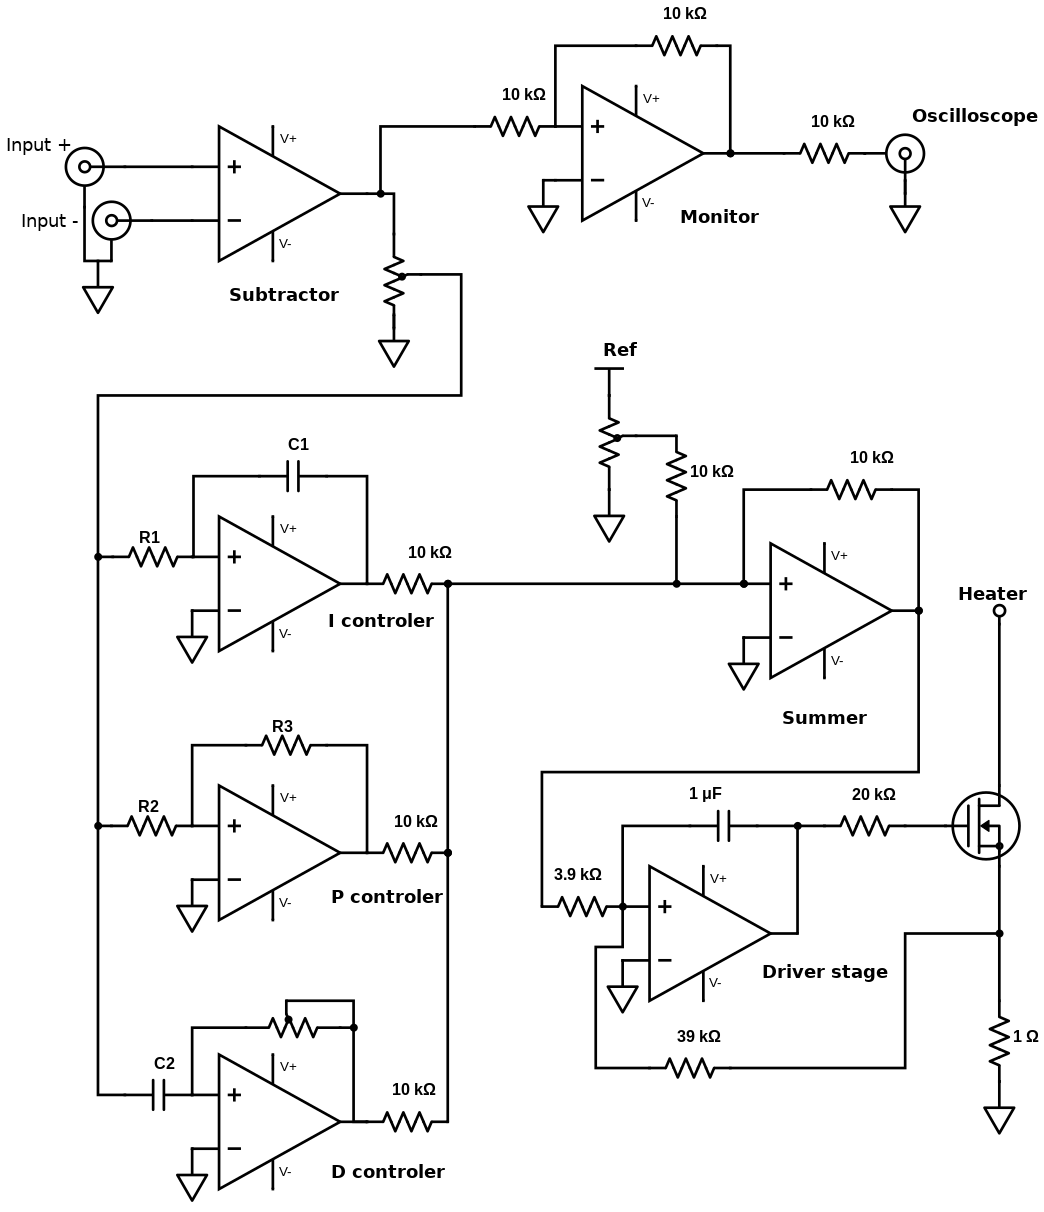
\includegraphics[width=0.8\textwidth]{circuit}
\caption{Complete schematic of the circuit, all the operation amplifiers and the instrumental amplifier were powered with +15 V and -15 V, moreover to every power pin we attached a 1 $\mu$F bypass capacitor. The Ref is also set to +15 V.}\label{circuit}
\end{figure}
\begin{figure}[H]
\centering
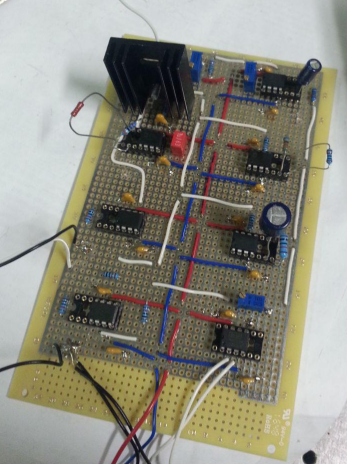
\includegraphics[width=0.4\textwidth]{photocircuit}
\caption{Photo of the realized circuit}\label{photocircuit}
\end{figure}
\section{Analysis}
\begin{figure}[H]
\centering
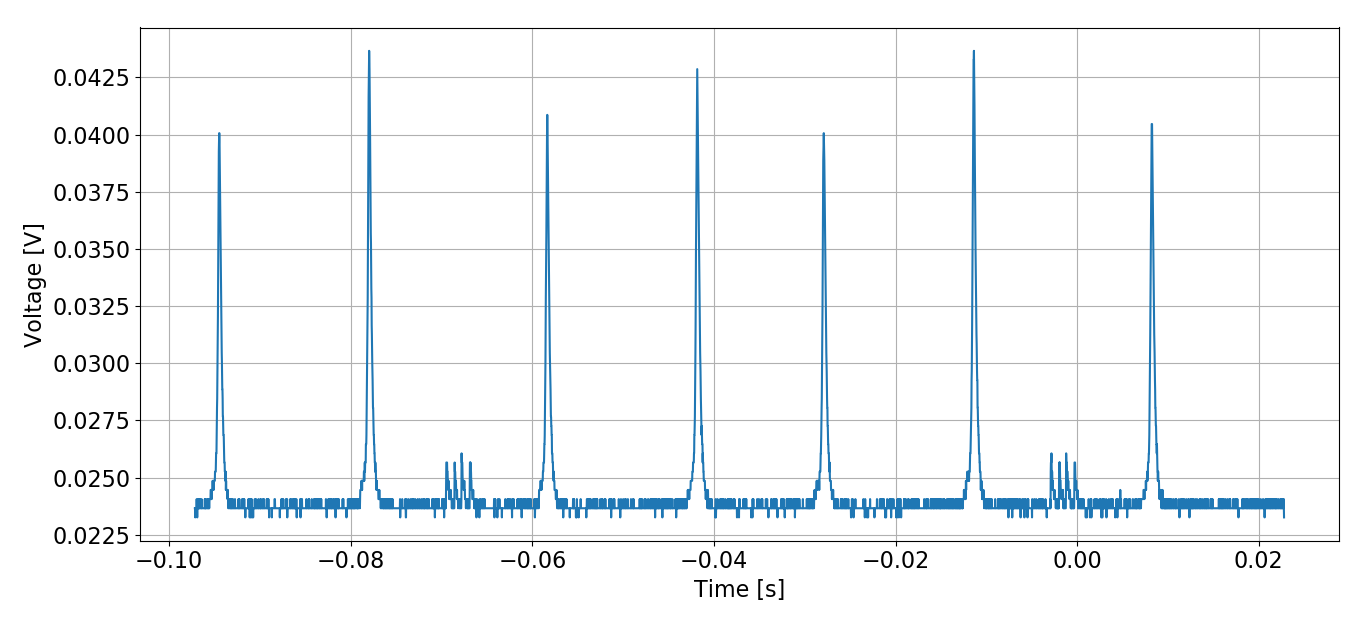
\includegraphics[width=\textwidth]{laser}
\caption{Output modes of the laser, not every peak is a mode, to identify the modes we need to look at peaks with approximately the same height, in this case the three highest peaks.}\label{laser}
\end{figure}
Before starting the analysis we have to change the time axis of the oscilloscope to frequency, such that we can analyze the frequency behaviour of the laser. This can be done knowing the free spectral range (FSR) of the laser, for the He-Ne laser used in this experiment the distance between two modes is 1.1 GHz \cite{script}. In figure \ref{laser} we can see the output of the He-Ne laser, by taking the distance in time between two modes we can find the factor A of conversion between time $t$ and frequency $f$
\[f = At, \qquad A = \frac{\text{FSR}_f}{\text{FSR}_t},\] 
where $\text{FSR}_f$ and $\text{FSR}_t$ are respectively the FSR measured in frequency and time. To find the peak we used a simple algorithm, where we took the point with the maximum value in the neighborhood.
To measure the stability of the laser, we changed the setting of the oscilloscope to persistence mode, which means that the oscilloscope adds a new measurement line per cycle, while still displaying old measurement lines. For every measurement we took a 2 minutes persistence trace of one peak of the laser, so we were able to analyze the laser stabilization over time. We took three measurements: in the first one, only the P controller was connected; in the second one we connected the P and the I controller; and for the last measurement we connected the whole PID controller. In figure \ref{fig_width_pid} the three measurements can be seen. To extract useful data from these images we used a image manipulation software to count the pixels of the FWHM for every peak, then we counted the pixel of one division, and knowing the division value in time is $1$ ms we are able to convert pixel to time. Finally from time we converted the values to frequency as described above. In the following table the results obtained are summarized
\begin{table}[H]
\centering
\begin{tabular}{l|c}

               & FWHM  {[}GHz{]} \\ \hline
P controller   & 0.035           \\ \hline
PI controller  & 0.014           \\ \hline
PID controller & 0.020           \\ \hline
\end{tabular}
\caption{Results obtained for the FWHM}
\end{table}
Unfortunately we do not have any error on these measurements, since the chosen analysis strategy did not allow us to perform a deep and precise analysis. Anyway we can clearly see an improvement from the P controller to the PI controller, but when we connected also the D controller, we apparently had a worse result as can be also seen in figure \ref{PID} where the persistence is broader then the previous case.

\begin{figure}[H]
  \centering{}
  \begin{subfigure}[t]{0.45 \textwidth}
    \centering
    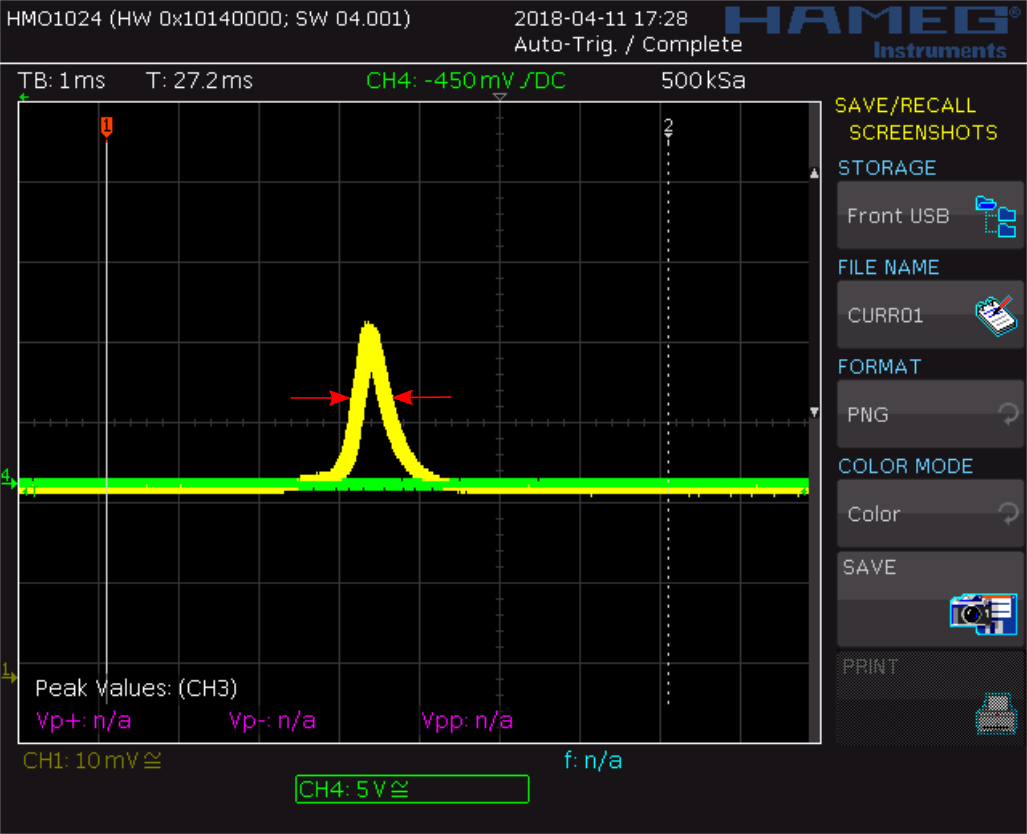
\includegraphics[height=6cm]{Pcontrolerpeak.png}
    \caption{With only the P controller }
  \end{subfigure}
  ~
  \begin{subfigure}[t]{0.45 \textwidth}
    \centering
    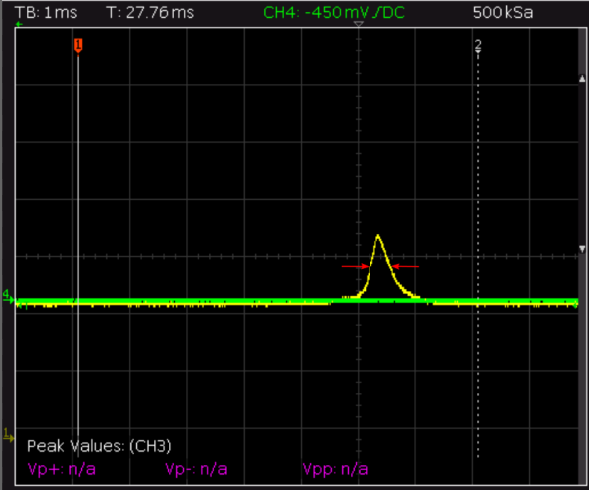
\includegraphics[height=6cm]{PIcontrolerpeak.png}
    \caption{PI controller }
  \end{subfigure}
  ~
  \begin{subfigure}[t]{0.45 \textwidth}
    \centering
    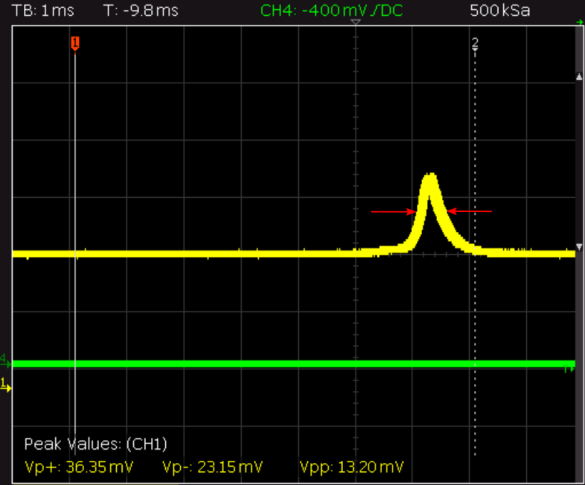
\includegraphics[height=6cm]{PIDcontrolerpeak.png}
    \caption{With the PID controller }\label{PID}
  \end{subfigure}
  \caption{Screenshot of the persistence measurements. Red arrows indicate where we measured the FWHM of the peaks.}
  \label{fig_width_pid}
\end{figure}

\section{Conclusion}
In this experiment we stabilized a laser using a PID controller, we tested the controller with only the proportional part, then using both the proportional and integral part, and finally we tested the whole PID controller. Our expectation was to have an improvement for very part of the controller that we used. However we noticed this behaviour for only the integral part, when we attached also the differential part, the mode of the laser was less stable. This can be due to a wrong choice of the capacitor $C_2$ or maybe some other problems with the circuit, which need further investigation.

\begin{thebibliography}{99}
\bibitem{script}
\textsc{H.C. Nägerl}, \textit{FP3 Versuch: Elektronischer Regler}, Universität Innsbruck

\bibitem{laserfaq}
\textsc{Samuel M. Goldwasser}, \textit{Sam's Laser FAQ}, \url{http://www.repairfaq.org/sam/laserhen.htm#henpolm}

\bibitem{halbleiter}
\textsc{U. Tietze, Ch. Schenk}, \textit{Halbleiter-Schaltungstechnik}, (12th edition) Springer-Verlag

\bibitem{ina114}
\textsc{Burr - Brown},\url{http://www.ti.com/lit/ds/symlink/ina114.pdf}

\bibitem{op27}
\textsc{Analog Devices}, \url{www.analog.com/media/en/technical-documentation/data-sheets/OP27.pdf}
\end{thebibliography}

\end{document}
